\documentclass[a4paper]{article}
\usepackage{multirow}
\usepackage{longtable}
\usepackage{graphicx}

\begin{document}

\subsubsection{CompareParentsEqualType}

  \begin{description}
  \item[testcase\_01:] Es werden 2 identische Modelle verglichen.    
  
  \textbf{Similarity:} 1
  
	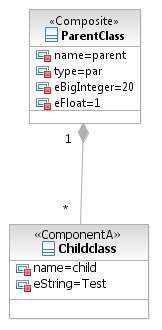
\includegraphics[scale=0.9]{CompareParentsEqualTypeTestScreens/Testcase01model1.jpeg}
	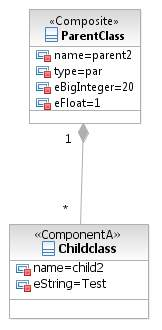
\includegraphics[scale=0.9]{CompareParentsEqualTypeTestScreens/Testcase01model2.jpeg}
	
  \item[testcase\_02:] Es werden 2 Modelle mit unterschiedlichen Typen beim Parent verglichen.
    
  \textbf{Similarity:} 0
  
	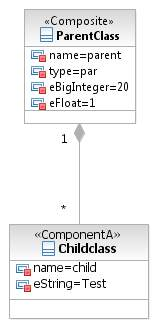
\includegraphics[scale=0.9]{CompareParentsEqualTypeTestScreens/Testcase02model1.jpeg}
	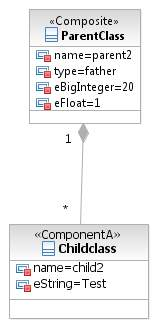
\includegraphics[scale=0.9]{CompareParentsEqualTypeTestScreens/Testcase02model2.jpeg}
	\end{description}


\end{document}